\toi{3.1}
\begin{wrapfigure}[9]{r}{0.4\linewidth}%
  \centering
  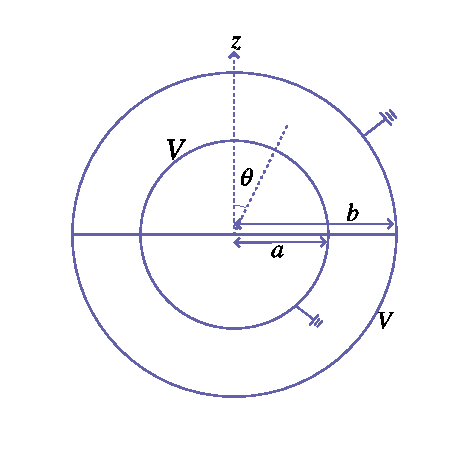
\includegraphics[width=\linewidth]{fig/Jackson3-1.pdf}%  
\end{wrapfigure}
半径$a, b$の球の間の領域のポテンシャルを考える.Legendre多項式による展開
\begin{gather}%
  \Phi(r, \theta) = \sum_{l=0}^\infty \ab(A_l r^l + B_l r^{-(l+1)}) P_l (\cos\theta)
\end{gather}
を以下の境界条件で考える:
\begin{gather}%  
  \label{eq:prob3-1_bc1}
  \Phi(a,\theta) =
  \begin{dcases}%
    V \qqtext{if} 0 \leq \theta \leq \frac{\pi}{2}\\
    0 \qqtext{if} \frac{\pi}{2} \leq \theta \leq \pi
  \end{dcases},\\
  \label{eq:prob3-1_bc2}
  \Phi(b,\theta) =
  \begin{dcases}%
    0 \qqtext{if} 0 \leq \theta \leq \frac{\pi}{2}\\
    V \qqtext{if} \frac{\pi}{2} \leq \theta \leq \pi
  \end{dcases}% 
\end{gather}%
\eqref{eq:prob3-1_bc1}について,$P_{l'}(\cos\theta)\dl{(\cos\theta)}$をかけて$\theta\in[0,\pi]$
で積分をすると,
\begin{multline}%
  \int_{\cos\theta=1}^{\cos\theta=-1} \sum_{l=0}^\infty\ab(A_la^l + B_la^{-(l+1)})
  P_l(\cos\theta) P_{l'}(\cos\theta) \dl{(\cos\theta)} \\
  =  V \int_{\cos\theta=1}^{\cos\theta=0} P_{l'}(\cos\theta) \dl{(\cos\theta)}
\end{multline}%
である.左辺の積分変数を$x$で書くと,
\begin{gather}%
  \text{(L.H.S.)} = \int_{1}^{-1} \sum_{l=0}^\infty\ab(A_l a^l + B_l a^{-(l+1)})
  P_l(x) P_{l'}(x) \dl{x}
\end{gather}
であり,Legendre多項式に関する直交関係\eqref{eq:legendre_ortho}より,($l,l'$を入れ替えて)
\begin{gather}%
  \label{eq:prob3-1_a}
  A_l a^l + B_l a^{-(l+1)} = \frac{V(2l+1)}{2} \int_0^1 \dl{x} P_l(x)
\end{gather}%
を得る.
同様に考えて,\eqref{eq:prob3-1_bc2}について,
\begin{gather}%
  \label{eq:prob3-1_b}
  A_l b^l + B_l b^{-(l+1)} =(-1)^l \frac{V(2l+1)}{2} \int_0^{1} \dl{x} P_l(x)
\end{gather}%
が成り立つ.
ただし,$P_l(-x) = (-1)^l P_l(x)$に注意せよ.

式\eqref{eq:prob3-1_a}と\eqref{eq:prob3-1_b}より,係数$A_l, B_l$を計算することができて,
\begin{gather}%
  A_l = \frac{(-1)^lb^{l+1}-a^{l+1}}{b^{2l+1}-a^{2l+1}}
  \frac{V(2l+1)}{2} \int_0^1 \dl{x} P_l(x),\\
  B_l = \frac{b^l-(-1)^la^l}{b^{2l+1}-a^{2l+1}}a^{l+1}b^{l+1}
  \frac{V(2l+1)}{2}\int_0^1 \dl{x} P_l(x)
\end{gather}%
がわかる.
したがって,ポテンシャルの正確な形は
\begin{multline}
  \Phi(r,\theta) =
  V \sum_{l=0}^\infty \ab(
  \frac{(-1)^lb^{l+1}-a^{l+1}}{b^{2l+1}-a^{2l+1}} r^l +
  \frac{b^l-(-1)^la^l}{b^{2l+1}-a^{2l+1}}a^{l+1}b^{l+1} r^{-(l+1)}
  )\\
  \times\frac{2l+1}{2}\ab(\int_0^1 \dl{x} P_l(x))
  P_l(\cos\theta)
\end{multline}

である.
具体的に$l = 4$の項までを書き下せば,
\begin{multline}
  \Phi(r,\theta) = V \left[
    \frac{1}{2} + \frac{3}{4}\frac{-(a^2+b^2)r+a^2b^2(a+b)r^{-2}}{b^3-a^3} P_1(\cos\theta)\right.\\
    \left.
    -\frac{7}{16}\frac{-(a^4+b^4)r^3 + a^4b^4(a^3+b^3)r^{-4}}{b^7-a^7}P_3(\cos\theta) +\cdots
    \right]
\end{multline}
となる.

$b \to \infty$の極限では$a/b \to 0, r/b\to 0$として,
\begin{align}%
  \Phi(r,\theta) 
  &= V
  \sum_{l=0}^\infty \frac{2l+1}{2}\ab(\frac{a}{r})^{l+1}
  \ab(\int_0^1\dl{x} P_l(x)) P_l(\cos\theta)\notag\\
  &= V\ab[
    \frac{1}{2} + \sum_{k=0}^\infty \frac{(-1)^k(4k+3)(2k-1)!!}{2^{k+2}(k+1)!} 
    \ab(\frac ar)^{2k+2} P_{2k+1}(\cos\theta)
  ]\\
  &= V\ab[
    \frac{1}{2} + \frac{3}{4}\ab(\frac{a}{r})^2 P_1(\cos\theta) -
    \frac{7}{16}\ab(\frac{a}{r})^4 P_3(\cos\theta) + \cdots
  ]
\end{align}%
である.
ただし,ここでは$(-1)!! = 1$と約束する.
これは半径$a$の導体球について,
北半球のポテンシャルが$V$,南半球が接地されており,さらに
無限遠でのポテンシャルの境界条件が$V/2$となる系において,導体球の外部領域に作る
ポテンシャルに等しいことがわかる.

$a \to 0$の極限では
\begin{align}%
  \Phi(r,\theta) &= V \sum_{l=0}^\infty (-1)^l \frac{2l+1}{2} \ab(\frac rb)^{l} 
  \ab(\int_0^1\dl{x} P_l(x)) P_l(\cos\theta)\notag\\
  &= V\ab[\frac 12 + \sum_{k=0}^\infty \frac{(-1)^{k+1}(4k+3)(2k-1)!!}{2^{k+2}(k+1)!}
  \ab(\frac rb)^{2k+1} P_{2k+1} (\cos\theta)]\\
  &= V\ab[\frac 12 - \frac 34 \ab(\frac rb) P_1(\cos\theta) +
  \frac{7}{16}\ab(\frac rb)^3P_3(\cos\theta)]
\end{align}%
である.
これは,半径$b$の導体球について,
北半球が接地されていて,南半球のポテンシャルが$V$となるような系における,
球内部のポテンシャルに等しいことがわかる.

それぞれの場合について,ポテンシャルを描く
と図\ref{fig:3-1_lima},\ref{fig:3-1_limb},\ref{fig:3-1_all}のようになる\footnote{
  描画のときに使用したコードは\texttt{.ipynb}形式で保存してある.
}.
\begin{figure*}[htbp]%  
  \centering%  
  \begin{minipage}{0.30\linewidth}
    \centering
    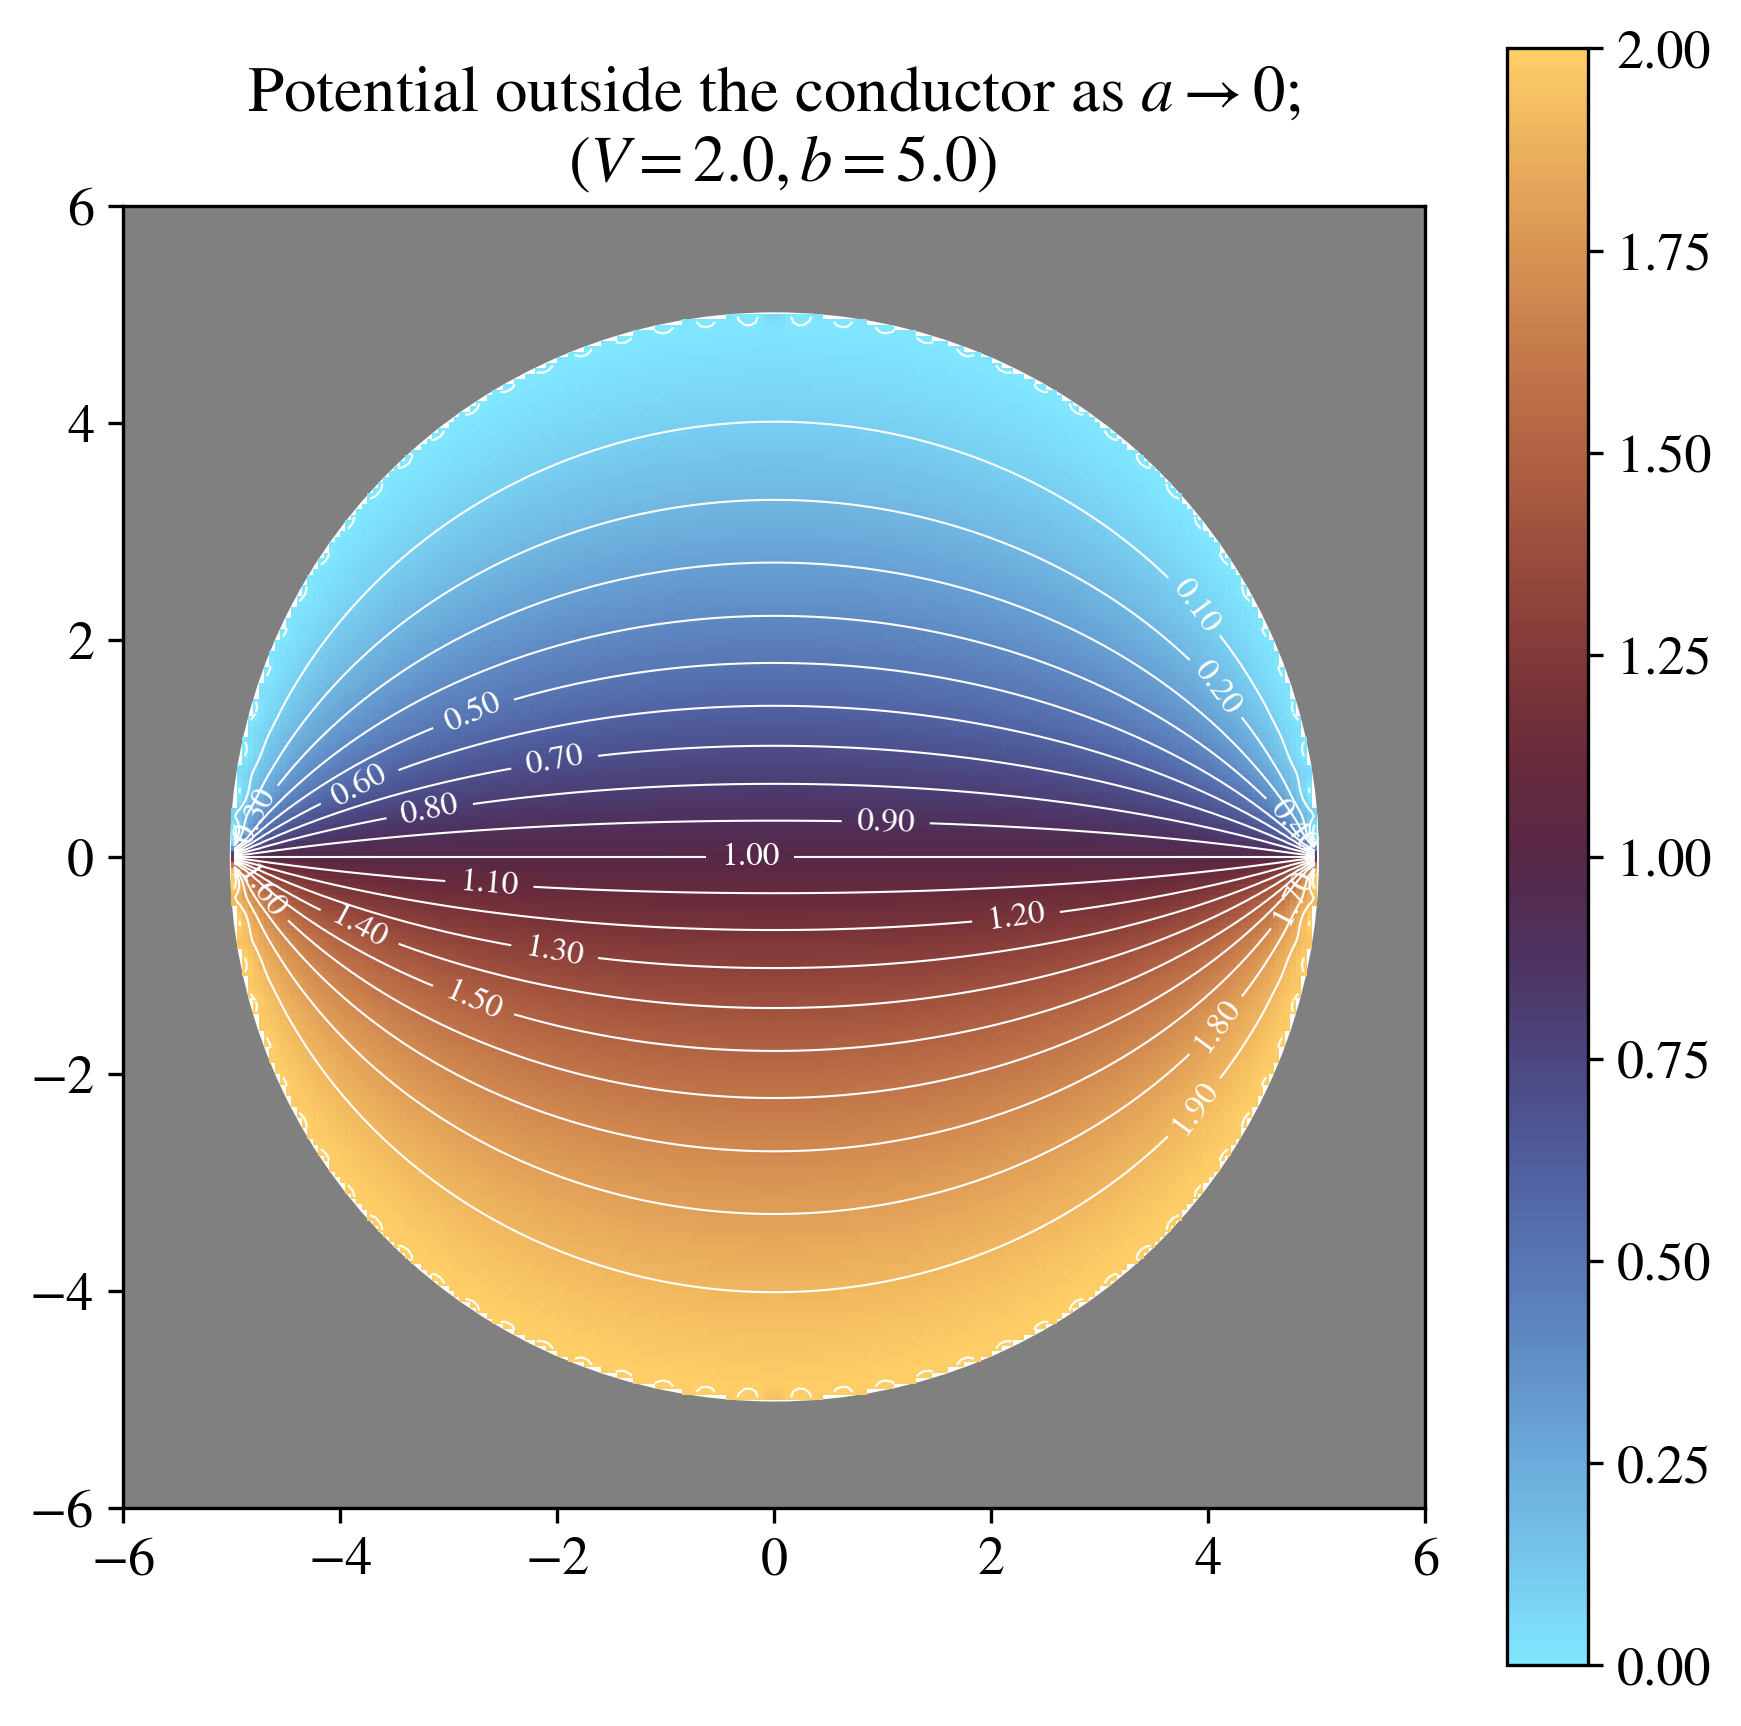
\includegraphics[width=\linewidth]{py/3-1_lima.png}%  
    \caption{$a \to 0$としたとき}%  
    \label{fig:3-1_lima}%  
  \end{minipage}
  \begin{minipage}{0.30\linewidth}
    \centering
    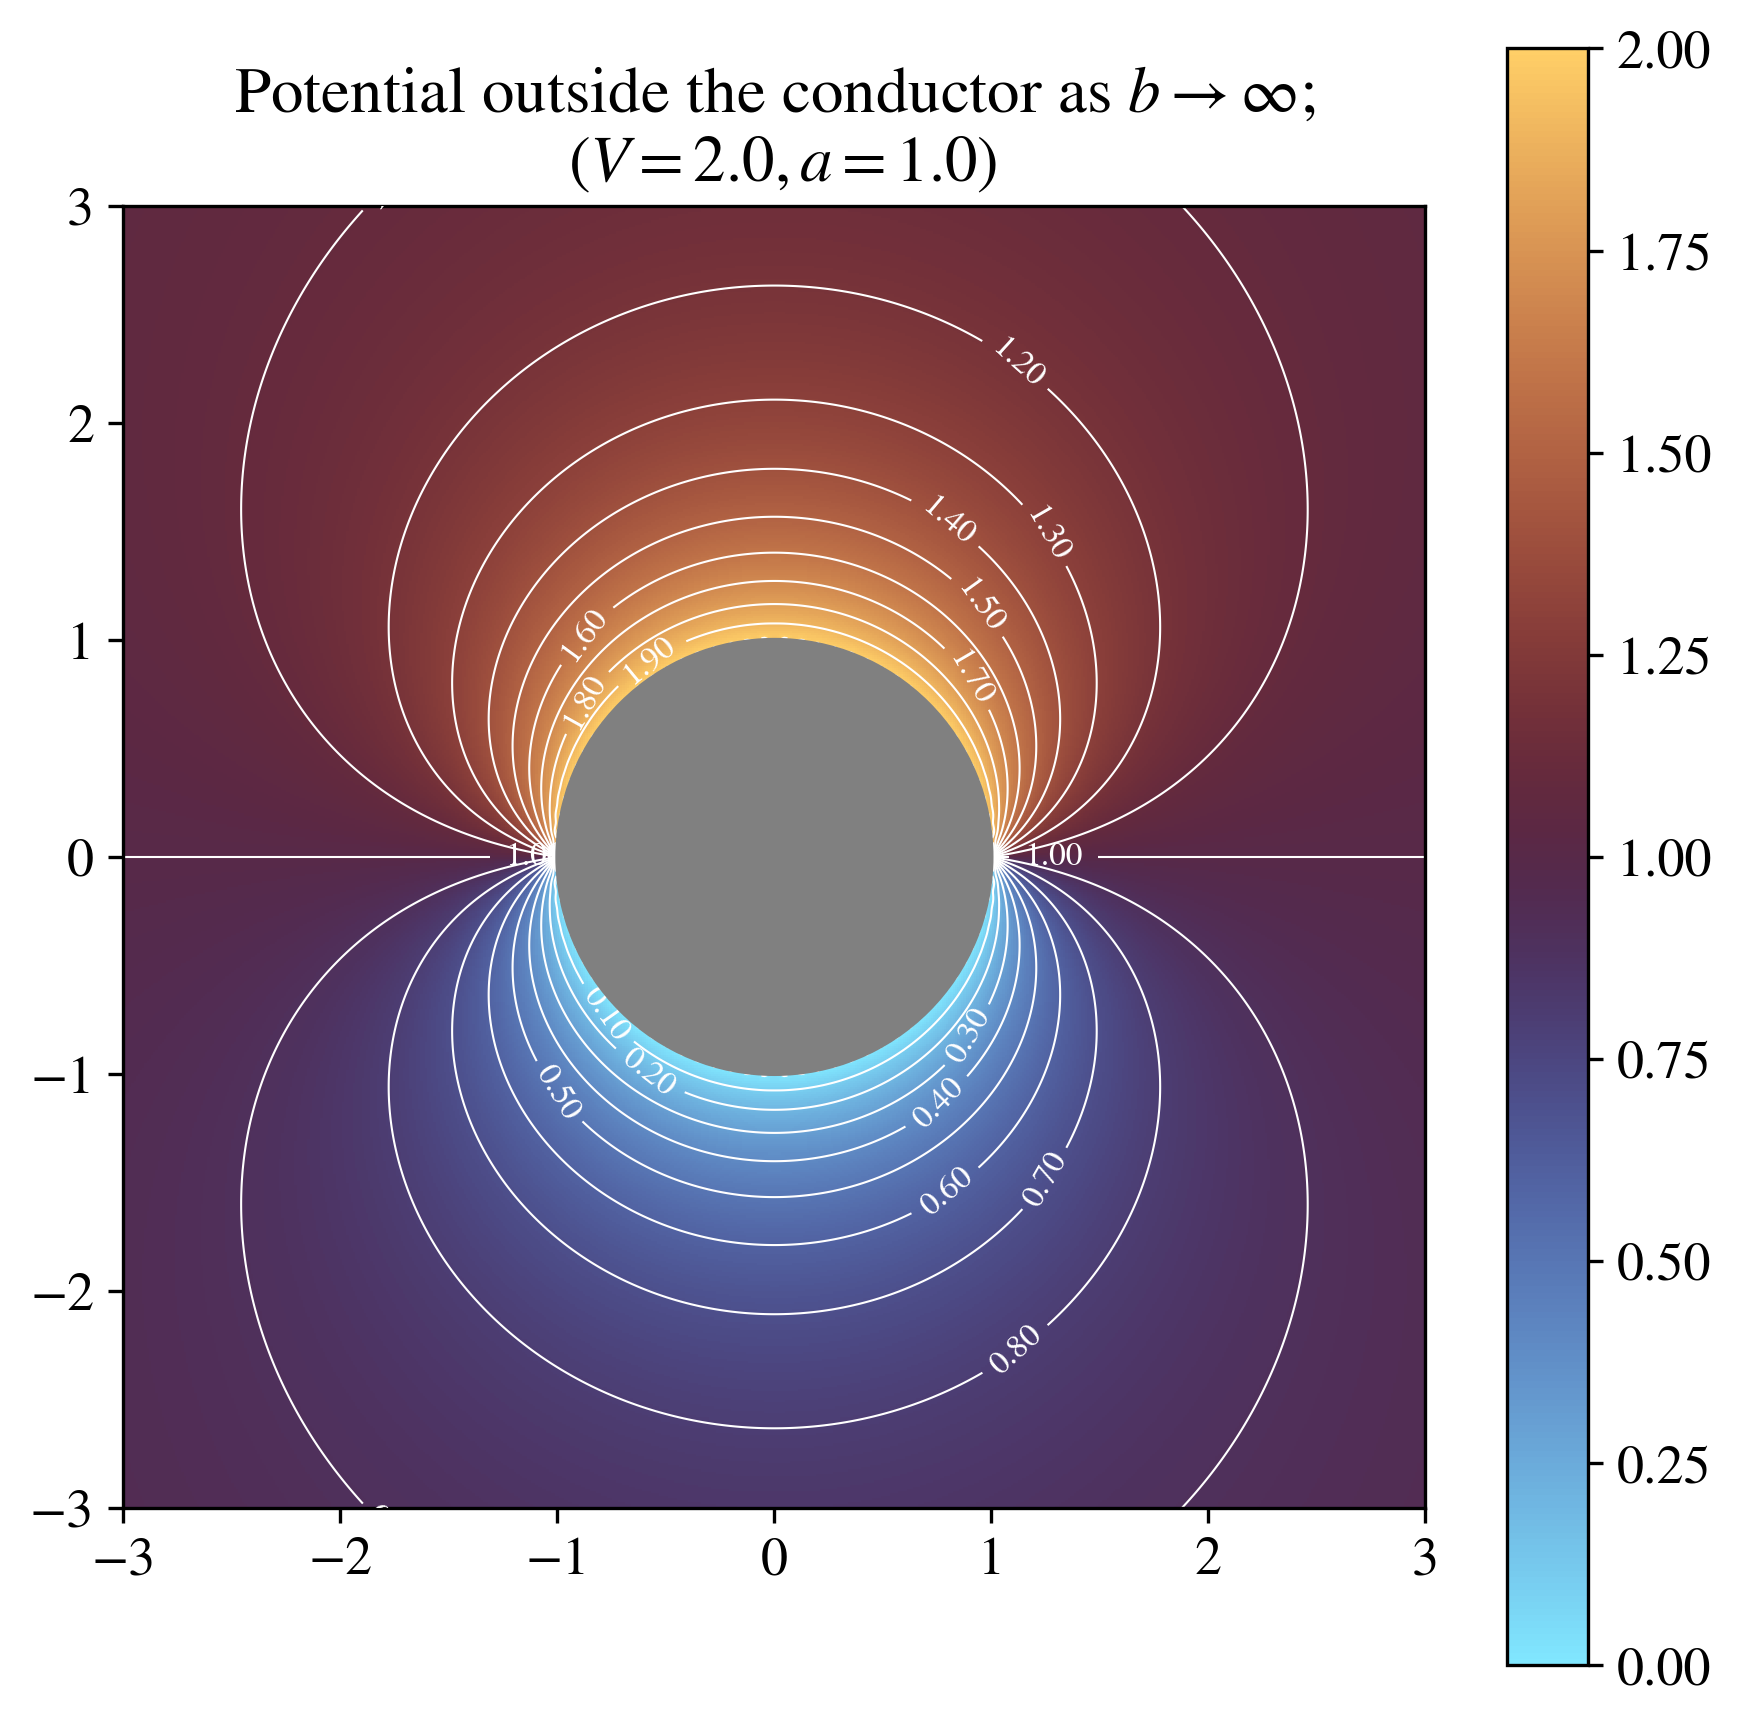
\includegraphics[width=\linewidth]{py/3-1_limb.png}%  
    \caption{$b\to\infty$としたとき}%  
    \label{fig:3-1_limb}%  
  \end{minipage}
  \begin{minipage}{0.30\linewidth}
    \centering
    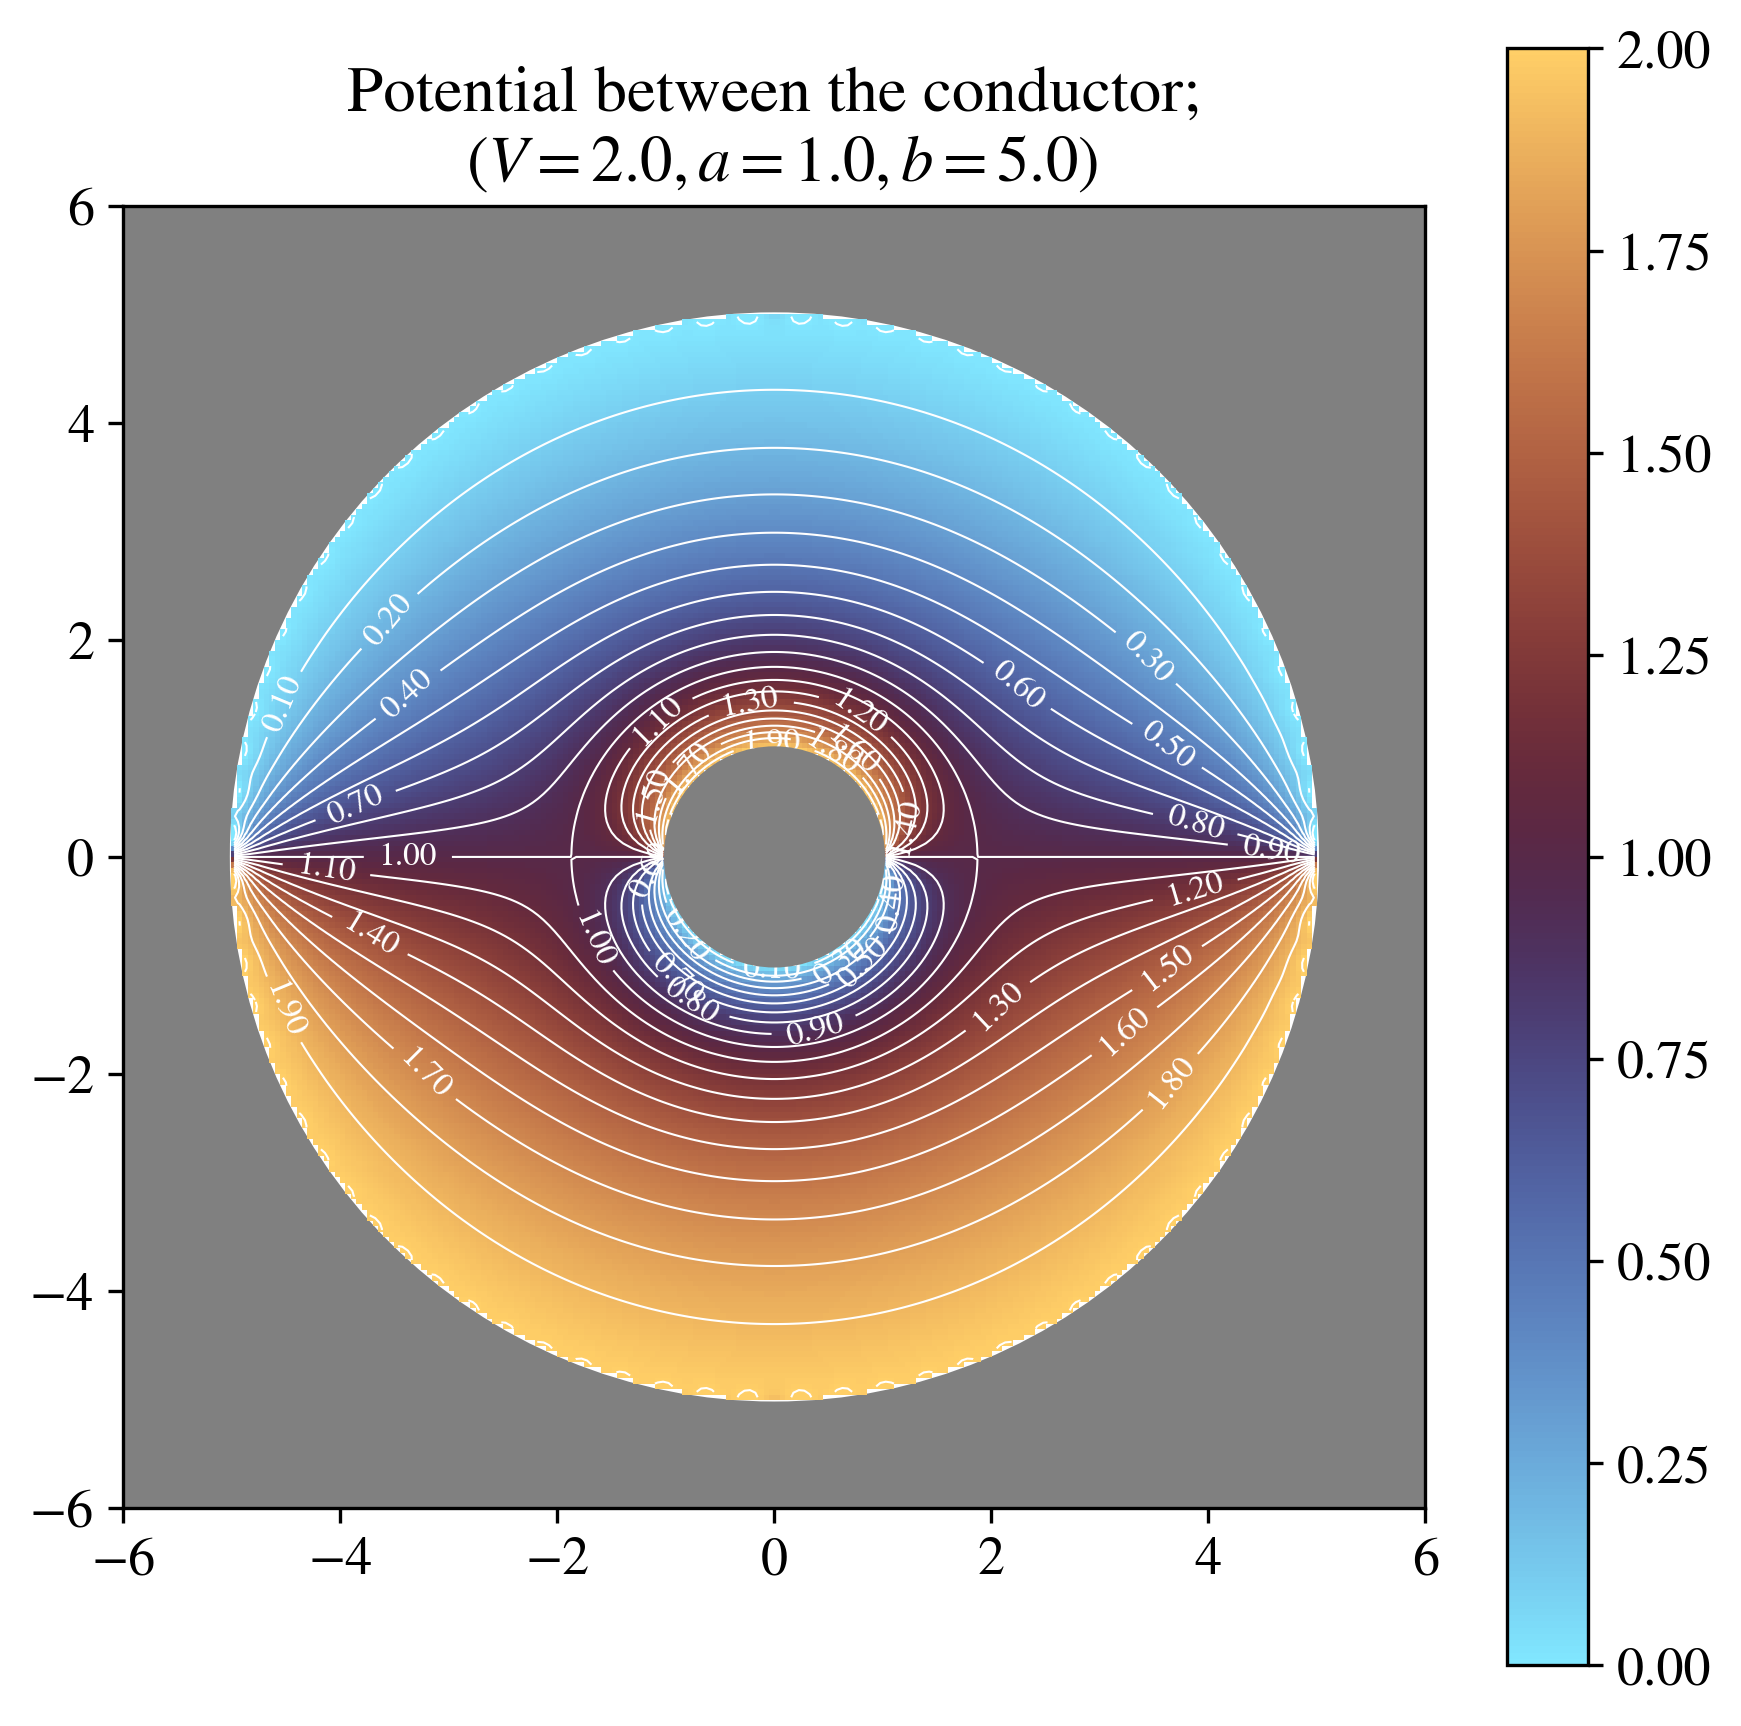
\includegraphics[width=\linewidth]{py/3-1_all.png}
    \caption{一般の場合についてのポテンシャル}
    \label{fig:3-1_all}
  \end{minipage}
\end{figure*}%


\hrulefill\\
%--- 問3.2 ---%
\toi{3.2}
\begin{wrapfigure}[10]{r}{0.35\linewidth}
  \centering%  
  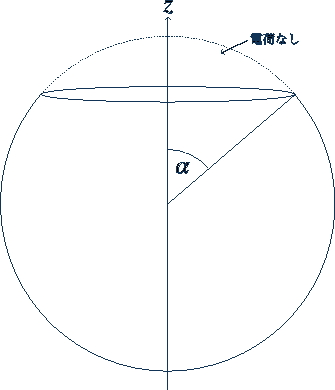
\includegraphics[width=\linewidth]{fig/Jackson3-2.pdf}%  
\end{wrapfigure}%
極角$\theta$が$\theta < \alpha$を満たす部分には電荷が存在せず,その他の部分には
一様な電荷密度$\sigma_{\mr{c}} = Q /(4\pi R^2)$が存在するような球を考える.

\itemlabel{(a)}
ポテンシャルをLegendre多項式で展開して
\begin{gather}%
  \Phi(r,\theta) = \sum_{l=0}^\infty \ab(A_l r^l + B_l r^{-(l+1)}) P_l(\cos\theta)
\end{gather}%
とする.
球の内部で$r\to 0$としたときに発散しない条件より$l = 0, 1, \ldots$について$B_l = 0$
また,球の外部については$r \to \infty$としたときにポテンシャルがゼロに漸近するとして,
$l = 0, 1, \ldots$について$A_l = 0$である.
したがって,球の内外でのポテンシャル$\Phi_{\text{in}}$および$\Phi_{\text{out}}$は
\begin{gather}%
  \Phi_{\text{in}}(r,\theta) = \sum_{l} A_l r^l P_l(\cos\theta),\\
  \Phi_{\text{out}}(r,\theta) = \sum_{l} B_l r^{-(l+1)} P_l(\cos\theta)
\end{gather}%
とかける.
ポテンシャルは$r= R$の球面上で連続であるから,
\begin{gather}%
  \sum_l A_l R^l P_l(\cos\theta) = \sum_l B_l R^{-(l+1)}P_l(\cos\theta)
\end{gather}%
であり,$\ab\{P_l\}_{l=0,1,2,\ldots}$が直交関数系をなすことより
$B_l = A_l R^{2l+1}$である.

また,電場の接続条件は
\begin{gather}%
  \sigma = \eps_0 \ab[\eval{\diffp{\Phi_{\text{in}}}{r}}_{r=R} -
  \eval{\diffp{\Phi_{\text{out}}}{r}}_{r=R}] 
  =
  \begin{dcases}%
    \frac{Q}{4\pi R^2} \qqtext{if} \theta \geq \alpha\\
    0 \qqtext{if} 0 \leq \theta < \alpha
  \end{dcases}%
\end{gather}%
である.
\begin{gather}%
  \eval{\diffp{\Phi_{\text{in}}}{r}}_{r=R}
  - \eval{\diffp{\Phi_{\text{out}}}{r}}_{r=R} 
  = \sum_{l=0}^\infty A_l \ab(2l+1) R^{l-1} P_l(\cos\theta)
\end{gather}%
に注意すると,$\dl{(\cos\theta)}P_{l'}(\cos\theta)$をかけて$\cos\theta =1$から
$\cos\theta = -1$で積分をすると,
直交関係より以下が得られる($l,l'$の入れ替えを行った);
\begin{gather}%
  A_l = \frac{Q}{8\pi \eps_0}\frac{1}{R^{l+1}} \int_{-1}^{\cos\alpha} \dl{x} P_l(x).
\end{gather}%
Legendre多項式に関する漸化式
\begin{gather}%
  \diff{P_{l+1}}{x} - \diff{P_{l-1}}{x} = (2l+1)P_l
\end{gather}%
より,
\begin{gather}%
  \int_{-1}^{\cos\alpha} \dl{x} P_l(x) 
  = \frac{1}{2l+1}\ab[P_{l+1}(\cos\alpha) - P_{l-1}(\cos\alpha)]
\end{gather}%
である($P_{l+1}(-1) - P_{l-1}(-1) = 0$であることに注意せよ).
したがって,
\begin{gather}%
  A_l = \frac{Q}{8\pi \eps_0} \frac{1}{2l+1} \ab[P_{l+1}(\cos\alpha) - P_{l-1}(\cos\alpha)]\frac{1}{R^{l+1}}
\end{gather}%
であり,球内部のポテンシャルは
\begin{gather}%
  \Phi_{\text{in}}(r,\theta) = \frac{Q}{8\pi \eps_0} \sum_{l=0}^\infty \frac{1}{2l+1}
  \ab[P_{l+1}(\cos\alpha) - P_{l-1}(\cos\alpha)] \frac{r^l}{R^{l+1}} P_l(\cos\theta)
\end{gather}%
と表される.
また,球外部のポテンシャルについては,
\begin{gather}%  
  \Phi_{\text{out}}(r,\theta) = \frac{Q}{8\pi \eps_0} \sum_{l=0}^\infty \frac{1}{2l+1}
  \ab[P_{l+1}(\cos\alpha) - P_{l-1}(\cos\alpha)] \frac{R^l}{r^{l+1}} P_l(\cos\theta)
\end{gather}%
と表される.

\itemlabel{(b)}
電場は$\bs{E} = -\gr \Phi$で与えられるので,
\begin{align}%  
  E_r &= -\diffp{\Phi}{r} \notag\\
  &= -\frac{Q}{8\pi \eps_0}\sum_{l=1}^\infty
  \frac{l}{2l+1}\ab[P_{l+1}(\cos\alpha) - P_{l-1}(\cos\alpha)] 
  \frac{r^{l-1}}{R^{l+1}} P_l(\cos\theta)\\
  E_\theta &= -\frac{1}{r}\diffp{\Phi}{\theta} \notag\\
  &= -\frac{1}{r}\frac{Q}{8\pi\eps_0} 
  \sum_{l=0}^\infty \frac{1}{2l+1} \ab[P_{l+1}(\cos\alpha) - P_{l-1}(\cos\alpha)]\frac{r^l}{R^{l+1}} \diff{P_l(\cos\theta)}{\theta}
\end{align}%
である.
原点では$r = 0$として考えると,$E_r, E_\theta$ともに$l=1$の項だけが残るので,
$P_2(\cos\alpha) - P_0(\cos\alpha) = -(3/2)\sin^2\al$であることなどに注意すると,
\begin{align}%
  \bs{E}(r=0) &= \frac{Q}{16\pi\eps_0}\frac{1}{R^2}\sin^2\alpha \ab[\cos\theta \hat{\bs{r}} - \sin\theta \hat{\bs{\theta}}] \notag\\
  &= \frac{Q}{16\pi \eps_0} \frac{1}{R^2}\sin^2\al \hat{\bs{z}}
\end{align}%
となる.

\itemlabel{(c-1-a)}
$\al \to 0$の極限を考える.

$\cos\al \sim 1 - \al^2 / 2$であるから,$P_l(\cos\al) \sim P_l(1) - (\al^2/2)P_l'(1)$として
Taylor展開できる.
$l = 0$のときは
\begin{gather}%
  P_1(\cos\al) - P_{-1}(\cos\al) = \cos\al + 1 \sim 2 - \frac{\al^2}{2}
\end{gather}%
$l \geq 1$のときは
\begin{align}%
  P_{l+1}(\cos\al) - P_{l-1}(\cos\al) 
  &\sim -\frac{\al^2}{2}\ab(P_{l+1}'(1) - P_{l-1}'(1))\notag\\
  &= -\frac{\al^2}{2}\ab(2l+1) P_l(1) = -\frac{2l+1}{2}\al^2
\end{align}%
と近似されるので,
\begin{align}%
  \Phi_{\text{in}} &\sim 
  \frac{Q}{4\pi \eps_0} \ab[\frac{1}{R} 
  - \frac{\al^2}{4}\sum_{l=0}^\infty \frac{r^l}{R^{l+1}}P_l(\cos\theta)]\notag\\
  &= \frac{Q}{4\pi\eps_0}\ab[
    \frac{1}{R} - \frac{\al^2}{4} \frac{1}{\ab|\bs{x} - R\hat{\bs{z}}|}
  ]
\end{align}%
とかける.
また,球外部のポテンシャルは
\begin{align}%
  \Phi_{\text{out}} &\sim \frac{Q}{4\pi\eps_0}\ab[
    \frac{1}{r} - \frac{\al^2}{4} \sum_{l=0}^\infty \frac{R^l}{r^{l+1}}P_l(\cos\theta)
  ]\notag\\
  &= \frac{Q}{4\pi\eps_0} \ab[
    \frac{1}{r} - \frac{\al^2}{4} \frac{1}{\ab|\bs{x} - R\hat{\bs{z}}|}
  ]
\end{align}%
であるから,球内外のポテンシャルは
\begin{gather}%
  \Phi \sim \frac{Q}{4\pi\eps_0} \ab[\frac{1}{r_>} - \frac{\al^2}{4}\frac{1}{\ab|\bs{x} - R \hat{\bs{z}}|}]
\end{gather}%
と統一的に書くことができる.ただし,$r_>$は$r$と$R$のうち大きい方である.

\itemlabel{(c-1-b)}
中心における電場の極限は$\sin\al \sim \al$に注意して
\begin{gather}%
  \bs{E}(r = 0) \sim \frac{Q}{16\pi \eps_0}\frac{\al^2}{R^2} \hat{\bs{z}}
\end{gather}%
である.

\itemlabel{(c-2-a)}
$\al \to \pi$の極限を考えるが,簡単のため$\beta \equiv \pi - \al \to 0$の極限を考える.
\begin{gather}%
  \cos\al = \cos(\pi -\be) \sim -1 + \frac{\be^2}{2}
\end{gather}%
に注意すると,(c-1)と同様にして,
\begin{gather}%
  P_{l+1}(\cos\al) - P_{l-1}(\cos\al) \sim (-1)^l \frac{2l+1}{2} \be^2
  \qqtext{for} l = 0, 1, \ldots
\end{gather}%
と表せる.したがって,
\begin{align}%
  \Phi_{\text{in}} &\sim \frac{Q}{8\pi\eps_0} \be^2
  \frac{1}{2} \sum_{l=0}^\infty (-1)^l \frac{r^l}{R^{l+1}} P_l(\cos\theta)\notag\\
  &= \frac{Q}{16\pi\eps_0}\beta^2 \sum_{l=0}^\infty \frac{r^l}{R^{l+1}} P_l(-\cos\theta)\notag\\
  &= \frac{Q}{16\pi\eps_0} \beta^2 \frac{1}{\ab|\bs{x} + R \hat{\bs{z}}|}
\end{align}%
である.球外のポテンシャルも同様に計算することができて,
\begin{gather}%
  \Phi_{\text{out}} \sim \frac{Q}{16\pi\eps_0} \beta^2 \frac{1}{\ab|\bs{x} + R \hat{\bs{z}}|}
\end{gather}%
となる(同じ結果を与える).

\itemlabel{(c-2-b)}
原点での電場は$\sin\al =\sin\be \sim \be$に注意して,
\begin{gather}%  
  \bs{E}(r=0) \sim \frac{Q}{16\pi\eps_0} \frac{\be^2}{R^2} \hat{\bs{z}}
\end{gather}%
と計算される.

\begin{tcolorbox}[dashedbox]%  
  (c-1)での結果について,これは,半径$R$の球表面に総電荷$Q$が分布しており,極角$\al$の部分には
  それに加えて,表面電荷密度$-\sigma = -Q/(4\pi R^2)$が分布している状況と一致している.
  具体的に計算をすると,まず総電荷$Q$が一様に分布しているとき,球内部のポテンシャルは
  簡単な計算により
  \begin{gather}%
    \Phi_{\text{in}}^{(1)} = \frac{Q}{4\pi\eps_0} \frac{1}{R}
  \end{gather}%
  であることがわかる.次に,極角$\al$の範囲については,$\al$が十分に小さいとき,
  この部分に存在する電荷は
  \begin{align}%
    \int \dl{\Omega}R^2(-\sigma) &= -2\pi R^2\sigma \int_0^\al \dl{\theta} \sin\theta\notag\\
    &= -2\pi R^2\sigma \ab(1-\cos\al) \notag\\
    &\sim -2\pi R^2 \sigma \frac{\al^2}{2} = -\frac{\al^2}{4}Q
  \end{align}%
  である.$\al$が十分に小さいとして,この電荷を点電荷とみなすことにすると
  これが作るポテンシャルは
  \begin{gather}%
    \Phi_{\text{in}}^{(2)} = -\frac{Q}{4\pi\eps_0} \frac{\al^2/4}{\ab|\bs{x}-R\hat{\bs{z}}|}
  \end{gather}%
  となり,$\Phi_{\text{in}}^{(1)} + \Phi_{\text{in}}^{(2)}$が(c-1-a)の
  答えになっていることが確かめられる.$\Phi_{\text{out}}$については$\Phi^{(1)}$の$1/R$を$1/r$
  として考えれば良く,この結果も整合的である.
\end{tcolorbox}
(a)で考えたポテンシャルを図示すると図\ref{fig:3-2_normal}のようになる.
\begin{figure}[H]%  
  \centering%  
  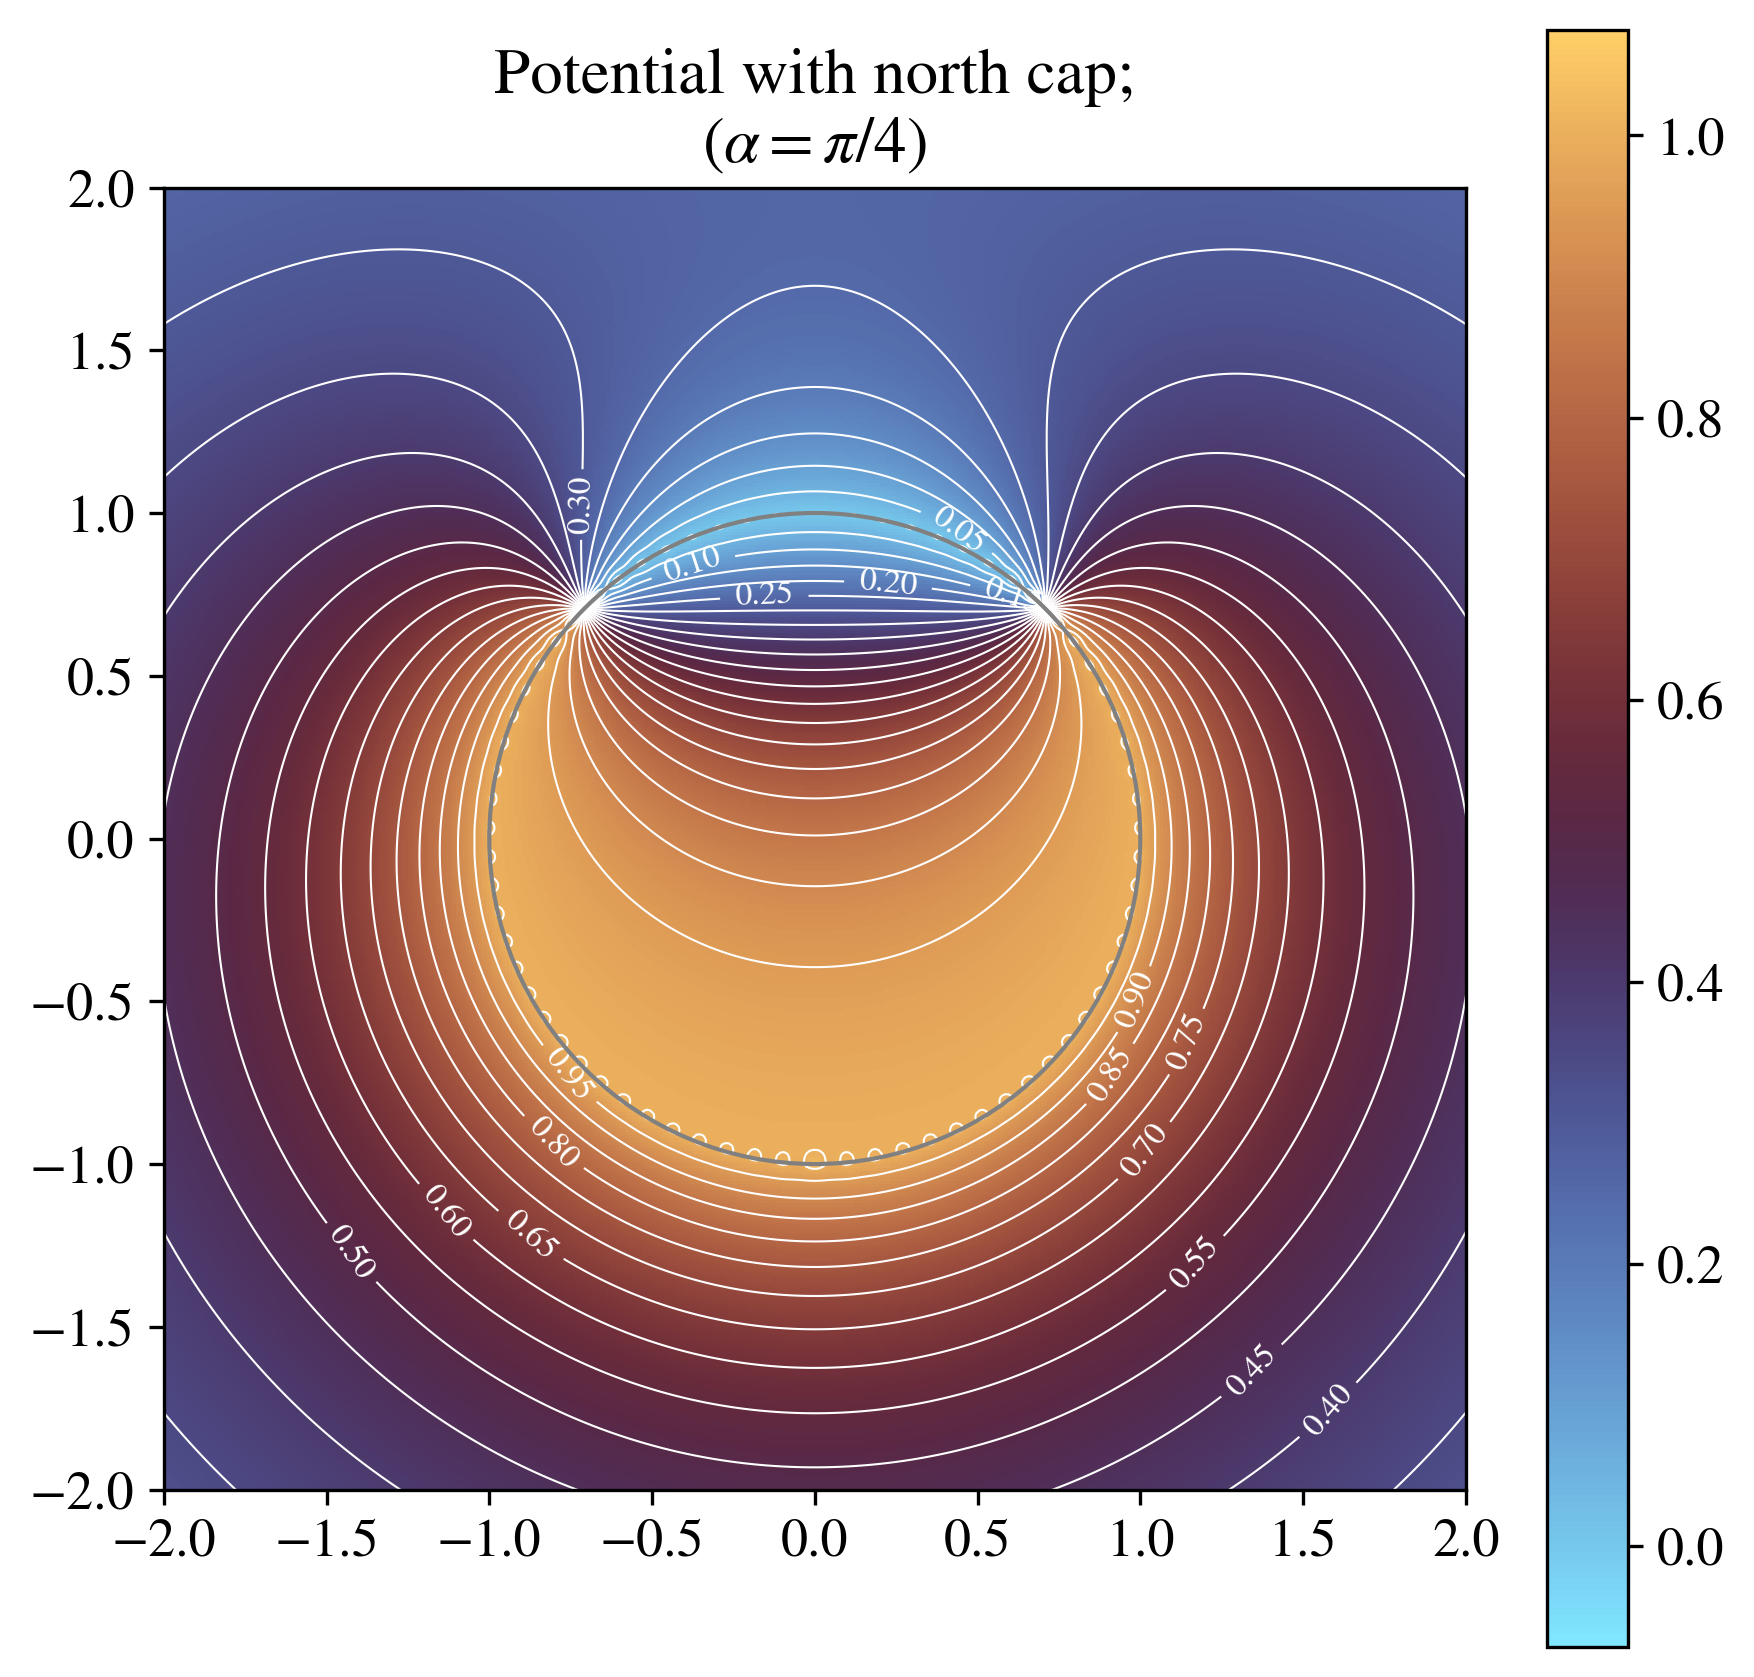
\includegraphics[width=0.8\linewidth]{py/3-2_normal.png}%  
  \caption{$\alpha = \pi/4$としてポテンシャルを描いた様子.
  ポテンシャルの単位は$Q/(4\pi\eps_0)$としており,球(図中の灰色の実線)
  の半径を$R = 1$としている.
  }%  
  \label{fig:3-2_normal}%  
\end{figure}%

\hrulefill\\
\toi{3.3}


